\chapter{Fundamentação Teórica}


\section{Sistemas de Controle}

Os sistemas de controle constituem um conjunto integrado de componentes que visam a regulação e a supervisão do
comportamento de sistemas dinâmicos.
Essenciais em uma muitas de aplicações práticas, são empregados para assegurar a estabilidade operacional e a precisão de resposta a perturbações.
A operação desses sistemas pode ser realizada sob duas configurações principais: sistemas de malha aberta,
onde não há realimentação do estado do sistema, e sistemas de malha fechada, que se caracterizam pela incorporação de
realimentação na estratégia de controle.
A eficiência de um sistema de controle é determinada pela sua habilidade em alcançar e sustentar um estado operacional
desejado, reduzindo desvios e oscilações indesejadas.
A precisão com que um sistema de controle atinge e mantém a saída desejada, apesar das flutuações nos parâmetros ou nas
condições ambientais, é um indicador crítico de seu desempenho \cite{ogata2010engenharia}.

Um sistema de controle em malha aberta opera sem a leitura de qualquer variável.
Nesse arranjo, o controlador atua baseado apenas no sinal de entrada, sem ajustar sua ação em resposta a distúrbios ou
variações na saída.
Um exemplo clássico é o controle de velocidade de um motor, onde a quantidade de combustível é ajustada apenas com base
na velocidade desejada, sem considerar a velocidade real do motor \cite{ogata2010engenharia}.

Em contraste, um sistema de controle em malha fechada inclui um ciclo de realimentação, onde a saída é continuamente
monitorada e comparada com o sinal de referência.
A diferença entre esses dois, conhecida como erro, é utilizada pelo controlador para ajustar o sinal de controle e,
assim, minimizar o erro \cite{ogata2010engenharia}.

\begin{figure}[H]
    \centering
    \caption{Diagrama de blocos de um sistema de malha fechada}
    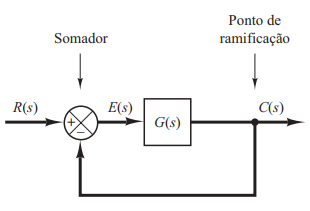
\includegraphics[scale=1]{figuras/closed_loop}
    \label{fig:closed_loop}
    \\
    \vspace{0cm}\hspace{0cm}\small{Fonte: \cite[Fig 2.3]{ogata2010engenharia}}
\end{figure}

Onde:
\begin{itemize}
    \item $R(s)$: Representa o sinal de referência.
    \item $G(s)$: Representa o sistema.
    \item $C(s)$: Representa a saída.
    \item $E(s)$: É o erro ou a diferença entre $R(s)$ e $C(s)$.
\end{itemize}

\subsection{Modelo}\label{subsec:modelfund}

De acordo com \cite{CoelhoIdentificacao}, em controle de processos, um modelo não busca ser uma réplica exata do
sistema real, mas sim uma representação adequada para uma aplicação específica.
A modelagem é um procedimento que visa obter um conjunto de equações matemáticas que descrevem a dinâmica do sistema,
permitindo responder a questões sobre o sistema sem a realização de experimentações físicas.
A simplicidade é muitas vezes uma virtude na modelagem de processos, pois modelos excessivamente complexos podem
não ser necessários para capturar a dinâmica essencial do sistema para fins de controle.

A função de transferência é uma forma comum de representar o modelo de um sistema em controle de processos.
Ela é definida como a razão entre a transformada de Laplace da saída e da entrada do sistema,
sendo uma razão de dois polinômios em $s$, onde $s$ é a variável complexa da transformada de Laplace.
Esta representação é particularmente útil para a análise e o projeto de sistemas de controle,
pois permite uma avaliação clara da resposta do sistema a diferentes tipos de sinais de entrada,
como impulso, degrau, rampa e senoidal.

Um modelo clássico e comumente utilizado para representação de sistemas de controle de primeira ordem com atraso é
representado pela seguinte função de transferência:
\begin{equation}
    \label{eq:firstordertf}
    G(s) = \frac{K}{\tau s + 1}e^{-\theta s}
\end{equation}
onde cada termo tem um significado específico:
\begin{itemize}
    \item $G(s)$: Função de transferência do sistema no domínio da frequência.
    \item $K$: Ganho do sistema, que determina a amplitude da saída em relação à entrada.
    \item $\tau$: Constante de tempo do sistema, que indica a rapidez com que o sistema responde a uma entrada.
    \item $\theta$: Tempo de atraso, que representa o tempo que leva para a resposta do sistema começar após uma entrada.
    \item $s$: Variável complexa da Transformada de Laplace, usada para transformar funções do tempo para o domínio da frequência.
\end{itemize}

Este modelo é particularmente útil para descrever sistemas onde há um atraso perceptível entre a ação de controle e a
resposta observada.
A exponencial negativa \( e^{-\theta s} \) incorpora o atraso no modelo, deslocando a resposta do sistema no tempo.
A constante de tempo \( \tau \) e o ganho \( K \) são parâmetros fundamentais que influenciam a dinâmica do sistema.
Por meio de simulações baseadas neste modelo, é possível prever o comportamento do sistema sob diferentes
condições operacionais e ajustar o projeto de um controlador antes da implementação real.

No contexto da automação industrial, os modelos matemáticos são empregados para previsão, análise e projeto de sistemas
de controle, essenciais para a sintonia de controladores e a otimização de processos.

\subsection{Controlador}

Dentro do universo dos sistemas de controle, um controlador é um componente crucial que modula a entrada de um sistema
para alcançar a saída desejada.
Ele atua ajustando o sinal de controle em resposta às variações da saída, visando minimizar a diferença entre a saída
observada e a saída desejada, conhecida como sinal de referência.
Os controladores podem ser classificados de acordo com suas ações de controle, alguns exemplos são controladores,
como on-off, proporcionais, integrais, proporcional-integrais (PI), proporcional-derivativos (PD) e
proporcional-integral-derivativos (PID), cada um com características distintas que os tornam adequados para diferentes
aplicações industriais \cite{ogata2010engenharia}.

%chck
O controlador PID é um dos tipos mais prevalentes de controladores em sistemas de controle, caracterizado pela sua
função de transferência,
\begin{equation}
    \label{eq:ctrlr}
    G_c(s) = K_p + \frac{K_i}{s} + K_d s
\end{equation}
onde \( K_p \), \( K_i \), e \( K_d \) representam os ganhos proporcional, integral e derivativo, respectivamente.
O termo proporcional \( K_p \) determina a reação do controlador à magnitude atual do erro,
o termo integral \( K_i \) acumula o erro ao longo do tempo, visando eliminar o erro estático,
e o termo derivativo \( K_d \) responde à taxa de variação do erro, antecipando o comportamento futuro.
A escolha adequada desses parâmetros é crucial: um \( K_p \) elevado pode acelerar a resposta do sistema, mas
potencialmente à custa da estabilidade;
um \( K_i \) excessivo pode introduzir oscilações devido ao atraso na resposta;
e um \( K_d \) significativo pode melhorar a estabilidade e a resposta rápida, mas é sensível ao ruído do sinal de
medição.
O ajuste dos três efeitos do controlador PID é essencial para otimizar o desempenho do sistema, tanto em resposta
transitória quanto em regime estacionário \cite{ogata2010engenharia}.

Vale ressaltar que controladores como P, PI e PD, podem ser vistos como um controlador PID onde o ganho para os
parâmetros não citados é ajustado para zero.

\subsection{Métodos de Identificação}

Segundo \cite{CoelhoIdentificacao}, métodos de identificação de sistemas referem-se ao conjunto de técnicas
utilizadas para construir modelos matemáticos que capturam a dinâmica de sistemas reais a partir de dados de entrada e
saída.
Estes métodos buscam determinar os parâmetros do sistema que melhor se ajustam às medidas observadas,
permitindo que o modelo matemático reproduza o comportamento do sistema.
A identificação pode ser conduzida de duas formas principais: \textit{off-line} e \textit{on-line}.

Na identificação \textit{off-line}, coleta-se um conjunto de dados de entrada e saída, comumente referidos como dados discretos,
processados posteriormente para estimar os parâmetros do modelo.
Este processo não possui restrições de tempo computacional e é tipicamente realizado utilizando algoritmos
não-recursivos.
Já a identificação \textit{on-line} ajusta os parâmetros do modelo em tempo real, sem a necessidade de armazenar previamente as
medidas.
Utiliza-se um algoritmo recursivo que atualiza os parâmetros após cada amostra coletada,
o que é particularmente útil para sistemas que mudam com o tempo ou quando é necessário um ajuste contínuo do modelo.

Devido ao escopo deste trabalho, métodos de identificação \textit{on-line} não serão abordados, apenas métodos \textit{off-line} baseados
nos dados discretos de resposta do sistema.

\subsubsection{Ziegler e Nichols}\label{subsubsec:znfun}

O método de Ziegler e Nichols é um clássico da literatura para identificação de modelos dinâmicos de
processos industriais.
Desenvolvido por Ziegler e Nichols em 1942 \cite{CoelhoIdentificacao}.

O processo de identificação de um modelo por esse método envolve a análise da resposta de um sistema a um sinal
degrau, para obter os parâmetros da equação\eqref{eq:firstordertf}, $K$, $\tau$ e $\theta$ e criar
a função de transferência representativa do modelo do sistema analisado.

Os parâmetros são calculados conforme indicado pela figura \ref{fig:zn_hg_ident_meth}.
\begin{figure}[H]
    \centering
    \caption{Métodos de ZN e HAG para a modelagem de processos de primeira ordem}
    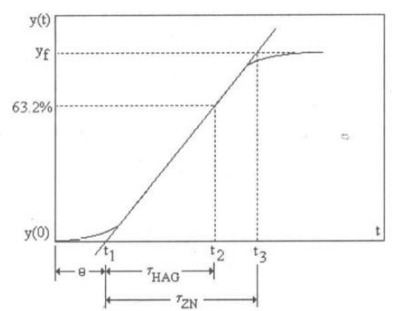
\includegraphics[scale=0.3]{figuras/zn_hg_ident_meth}
    \label{fig:zn_hg_ident_meth}
    \\
    \vspace{0cm}\hspace{0cm}\small{Fonte: \cite{CoelhoIdentificacao}}
\end{figure}

A reta traçada corresponde à tangente no ponto de máxima inclinação da curva de reação.

A constante de tempo $\tau$ é determinada pelo intervalo de tempo entre $t_1$, e o instante
$t_3$, onde a reta tangente toca o eixo $t$, e onde cruza com a reta $y(t) = y_f$,
respectivamente.
O valor de  $\theta$ é considerado como $t_1$, o intervalo entre a aplicação do sinal degrau e o
momento em que a reta tangente toca o eixo $t$.
Por fim, o valor de $K$ pode ser obtido a través da equação,
\begin{equation}
    \label{eq:dydu}
    K = \frac{\Delta y}{\Delta u}
\end{equation}
Ou seja $y_f$ dividido pelo valor do sinal degrau \cite{CoelhoIdentificacao}.

\subsubsection{Hägglund}\label{subsubsec:hagfun}

O método Hägglund é mais um clássico da literatura para identificação de modelos dinâmicos de
processos industriais.
Desenvolvido por Hägglund em 1991 \cite{CoelhoIdentificacao}.

A identificação de modelo pelo método de Hägglund é muito similar a de Ziegler e Nichols (\ref{subsubsec:znfun}), com a única diferença sendo que $\tau$ é determinado pelo intervalo de tempo entre $t_1$, e o instante $t_2$, sendo $t_2$
o momento em que a curva de resposta alcança o valor $y(t) = y(0) + 0.632y_f$, ou seja, $63.2\%$ do valor de regime.
Isso pode ser visualizado na figura \ref{fig:zn_hg_ident_meth}.

\subsubsection{Smith}\label{subsubsec:smfun}

Desenvolvido por Smith em 1985, o método Smith, assim como os métodos Hägglund e Ziegler-Nichols, busca encontrar
valores para os parâmetros $K$, $\tau$ e $\theta$ e criar a função de transferência representativa do modelo do sistema
analisado \cite{CoelhoIdentificacao}.

\begin{figure}[H]
    \centering
    \caption{Método de Smith para a modelagem de processos de primeira ordem}
    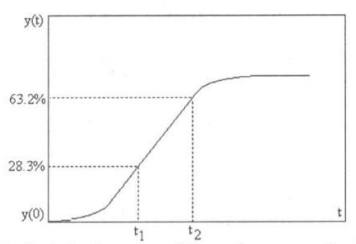
\includegraphics[scale=0.3]{figuras/sm_ident_meth}
    \label{fig:sm_ident_meth}
    \\
    \vspace{0cm}\hspace{0cm}\small{Fonte: \cite{CoelhoIdentificacao}}
\end{figure}

Na figura \ref{fig:sm_ident_meth} podem ser observados os momentos $t_1$ e $t_2$, eles correspondem a passagem da resposta
pelos pontos $y(t) = y(0) + 0.283y(\infty)$ e $y(t) = y(0) + 0.632y(\infty)$, respectivamente.

As constantes podem então ser utilizadas para o cálculo da constante de tempo $\tau$ e do valor de $\theta$,
conforme as seguintes equações:
\begin{equation}
    \label{eq:smtau}
    \tau = 1.5*(t_2 - t_1)
\end{equation}
\begin{equation}
    \label{eq:smtheta}
    \theta = t_2 - \tau
\end{equation}

Por fim o valor de $K$ pode ser obtido através da equação \eqref{eq:dydu}.

\subsubsection{Sundaresan e Krishnaswamy}\label{subsubsec:skfun}

O método de Sundaresan e Krishnaswamy, desenvolvido em 1977, é bastante similar ao método Smith \ref{subsubsec:smfun}.
Apresentando algumas alterações nos valores para o cácluculo das constantes de tempo $t_1$ e $t_2$, calculadas como
$y(t) = y(0) + 0.353y(\infty)$ e $y(t) = y(0) + 0.853y(\infty)$, respectivamente, como pode ser visto na figura
\ref{fig:sd_kr_ident_meth} \cite{CoelhoIdentificacao}:


\begin{figure}[H]
    \centering
    \caption{Método de Sundaresan e Krishnaswamy para a modelagem de processos de primeira ordem }
    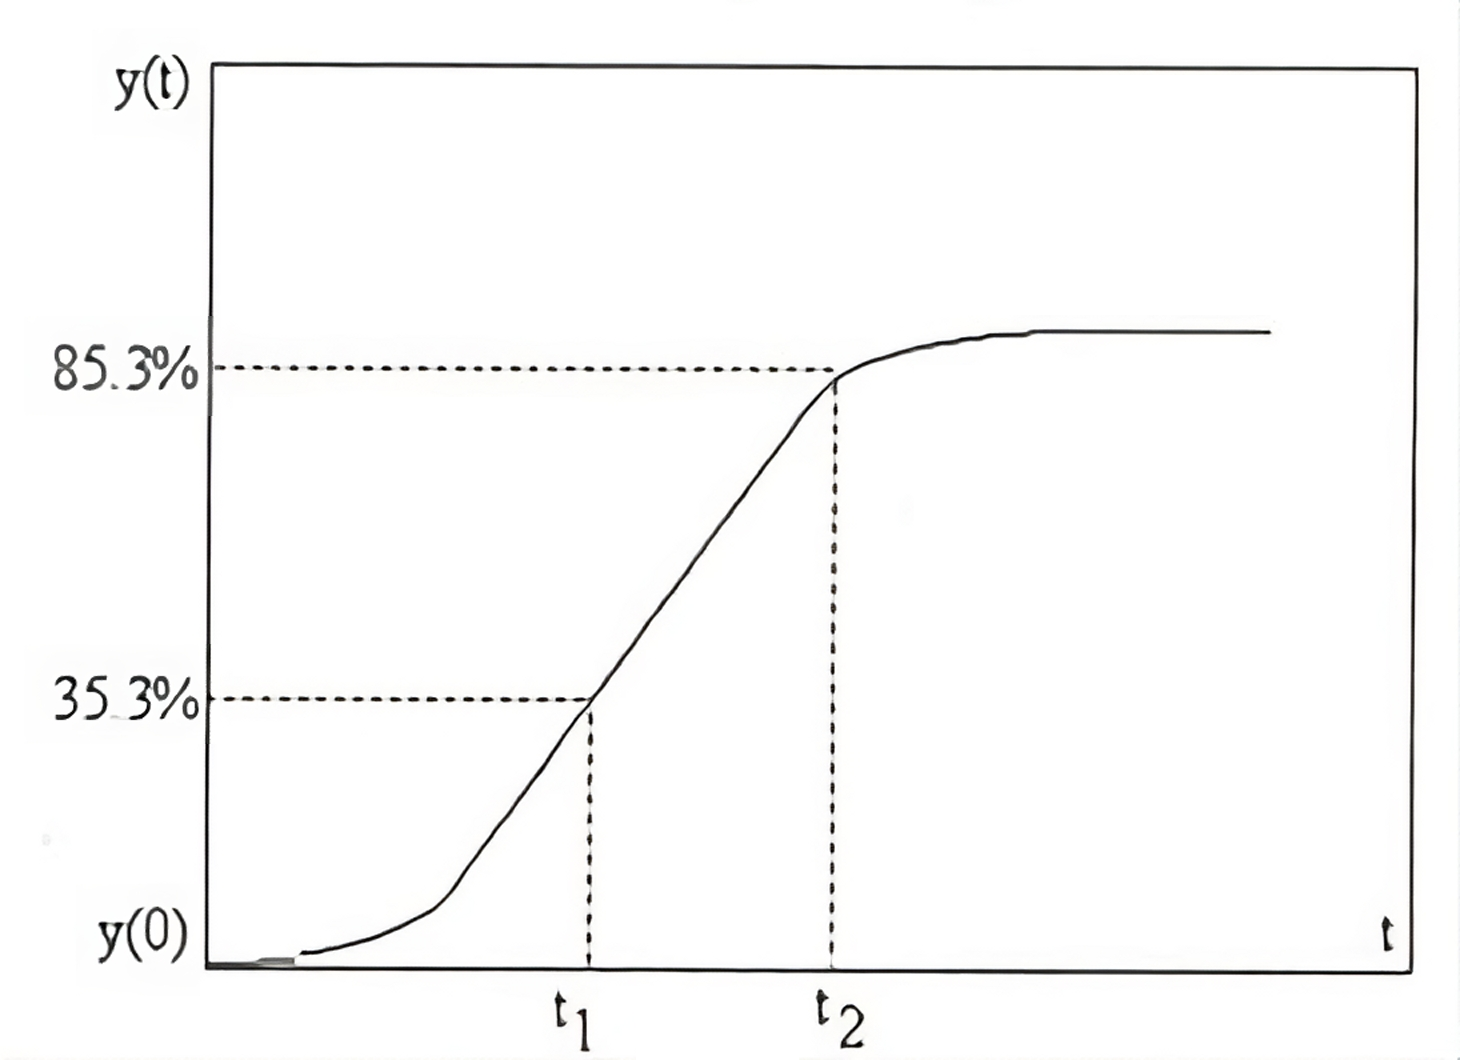
\includegraphics[scale=0.3]{figuras/sd_kr_ident_meth}
    \label{fig:sd_kr_ident_meth}
    \\
    \vspace{0cm}\hspace{0cm}\small{Fonte: \cite{CoelhoIdentificacao}}
\end{figure}

Além disso, o cálculo dos parâmetros $\tau$ e $\theta$ também tem diferenças,
para este método os parâmetros podem ser obtidos pelas equações \eqref{eq:sktau} e
\eqref{eq:sktheta}, respectivamente.
\begin{equation}
    \label{eq:sktau}
    \tau = 0.67*(t_2 - t_1)
\end{equation}
\begin{equation}
    \label{eq:sktheta}
    \theta = 1.3t_1 - 0.29t_2
\end{equation}

\subsubsection{Nishikawa}\label{subsubsec:nkfun}

Um último método clássico da literatura para Identificação de modelos é o desenvolvido por Nishikawa em 1984.
A pesar de buscar os mesmos parâmetros que os métodos anteriores, estes parâmetros são obtidos por meio de áreas
delimitadas pela curva de resposta a sinal degrau, pelo valor de regime e pela constante de tempo $t_0$, como pode ser
observado na figura \ref{fig:ni_ident_meth}.


\begin{figure}[H]
    \centering
    \caption{Método de Nishikawa para a modelagem de processos de primeira ordem}
    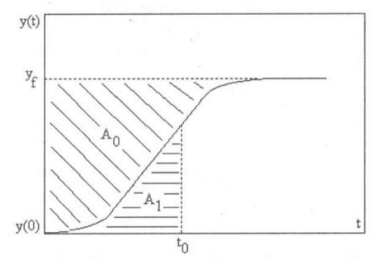
\includegraphics[scale=0.3]{figuras/ni_ident_meth}
    \label{fig:ni_ident_meth}
    \\
    \vspace{0cm}\hspace{0cm}\small{Fonte: \cite{CoelhoIdentificacao}}
\end{figure}

As áreas e a constante de tempo podem ser calculadas conforme as seguintes equações:

\begin{equation}
    \label{eq:nia0}
    A_0 = \int_{0}^{\infty} { \Delta y(\infty) - \Delta y(t) } dt
\end{equation}
\begin{equation}
    \label{eq:nia1nt0}
    A_1 = \int_{0}^{t_0} \Delta y(t) dt \;\; ; \;\; t_0 = \frac{A_0}{\Delta y(\infty)}
\end{equation}

Com isto, podem ser obtidas as constantes $\tau$ e $\theta$:
\begin{equation}
    \label{eq:nitau}
    \tau = \frac{A_1}{0.368\Delta y(\infty)}
\end{equation}
\begin{equation}
    \label{eq:nitheta}
    \theta = t_0 - \tau
\end{equation}

Da mesma forma que os outros métodos, $K$ pode ser obtido através da equação \eqref{eq:dydu}.

\subsection{Métodos de Aproximação de Controlador PID}

A sintonia de controladores PID é um componente crucial no desenvolvimento de sistemas de controle automatizados,
fundamental para assegurar a eficiência e a estabilidade operacional.
A importância da sintonia reside na sua capacidade de ajustar o comportamento do sistema de controle para atender às
especificações de desempenho, como precisão, rapidez de resposta e estabilidade a longo prazo.
A sintonia adequada consegue compensar as incertezas inerentes ao modelo do sistema e as variações ambientais,
garantindo que o sistema mantenha seu desempenho ótimo sob uma gama de condições operacionais.
\cite{apostpidsint}.

Realizar a sintonia de um controlador PID envolve a aproximação dos ganhos do controlador capazes de causar o efeito no
sistema.
Para isso é comumente feita a análise o modelo do sistema a ser controlado.
Através da análise do modelo, é possível prever como o sistema responde a diferentes configurações de controle e
identificar os parâmetros de ganho que resultarão na resposta desejada.
Este processo de aproximação dos ganhos, permite a sintonia do sistema, assegurando que o controlador PID opere de forma
eficiente, mantendo a saída do sistema nos parâmetros desejados, minimizando o erro e otimizando a resposta a
perturbações \cite{apostpidsint}.

\subsubsection{Controlador Z-N}\label{subsubsec:znctr}

Proposto por Ziegler e Nichols, como uma forma de obter os ganhos de controlador para os modelos identificados
pelo seu método de identificação (\ref{subsubsec:znfun}), o objetivo deste método é obter parâmetros de ganho PID que
façam a sintonia do controlador \cite{apostpidsint}.

Em específico, este método se baseia na curva de reação do sistema a resposta de sinal degrau, que é
exatamente o que o resultado da identificação por Ziegler Nichols obtém, utilizando os parâmetros $K$, $\tau$ e $\theta$
para análise.

Desta forma, são aplicadas as fórmulas do método conforme a tabela \ref{tab:zncntb}.

\begin{table}[h]
    \begin{center}
        \begin{tabular}{ | l | c | c | c | }
            \hline
            {\textbf{Controlador}} & {$K_P$}                               & {$T_I$}                & {$T_D$}       \\
            \hline
            {\textbf{P}}           & {$\frac{1}{K}\frac{\tau}{\theta}$}    & {$\infty$}             & {$0$}         \\
            \hline
            {\textbf{PI}}          & {$0.9\frac{1}{K}\frac{\tau}{\theta}$} & {$\frac{\theta}{0.3}$} & {$0$}         \\
            \hline
            {\textbf{PID}}         & {$1.2\frac{1}{K}\frac{\tau}{\theta}$} & {$2\theta$}            & {$0.5\theta$} \\
            \hline
        \end{tabular}
        \caption{Método de Ziegler e Nichols para Curva de Reação}
        \label{tab:zncntb}
    \end{center}
\end{table}

Os valores de $T_I$ e $T_D$ são $1/K_i$ e $1/K_d$, respectivamente.

\subsubsection{Controlador C-C}\label{subsubsec:ccapx}

Criado por Cohen e Coon como uma forma de obter os ganhos de controlador, de forma similar ao método de Ziegler e Nichols
(\ref{subsubsec:znctr}), para modelos clássicos de primeira ordem com atraso.
Utiliza a seguinte tabela para determinar os ganhos de controlador PID:

\begin{table}[h]
    \begin{center}
        \begin{tabular}{ | l | c | c | c | }
            \hline
            {\textbf{Controlador}} & {$K_P$}                               & {$T_I$}                & {$T_D$}       \\
            \hline
            {\textbf{P}}           & {$\frac{1}{K}\frac{\tau}{\theta}[1+\frac{\theta}{3\tau}]$}    & {$\infty$}             & {$0$}         \\
            \hline
            {\textbf{PI}}          & {$\frac{1}{K}\frac{\tau}{\theta}[0.9+\frac{\theta}{12\tau}]$} & {$\frac{\theta [30+3 \frac{\theta}{\tau}]}{9+20 \frac{\theta}{\tau}}$} & {$0$}         \\
            \hline
            {\textbf{PID}}         & {$\frac{1}{K}\frac{\tau}{\theta}[\frac{16\tau+3\theta}{12\tau}]$} & {$\frac{\theta [32+6 \frac{\theta}{\tau}]}{13+8 \frac{\theta}{\tau}}$}            & {$\frac{4 \theta}{11+2 \frac{\theta}{\tau}}$} \\
            \hline
        \end{tabular}
        \caption{Método de Cohen e Coon para Curva de Reação}
        \label{tab:cccntb}
    \end{center}
\end{table}

Os valores de $T_I$ e $T_D$ são $1/K_i$ e $1/K_d$, respectivamente.

\section{Implementação em {Python}}

\subsection{Bibliotecas em {Python}}

\abreviatura{pip}{package installer for Python}

No ecossistema de programação {Python}, bibliotecas desempenham um papel fundamental, servindo como repositórios ricos de
funções e métodos pré-construídos que permitem aos desenvolvedores executar uma gama ampla de tarefas com eficiência e
precisão.
Essas bibliotecas podem variar em seu escopo e aplicação, abrangendo desde operações matemáticas complexas, como as
oferecidas pelo NumPy, até a manipulação avançada de dados com o pandas, e interações de rede simplificadas através da
biblioteca requests.
A habilidade de reutilizar e adaptar código pré-existente não apenas acelera o processo de desenvolvimento, mas também
assegura a adesão a padrões de código testados e confiáveis \cite{pipy,pydocs} .

A ferramenta pip (package installer for Python) e o Python Package Index (PyPI) são componentes centrais na gestão e instalação de bibliotecas {Python}.
O pip, recomendado pela {Python} Packaging Authority (PyPA), é essencial para a instalação de pacotes {Python},
facilitando a integração de bibliotecas de terceiros em projetos de desenvolvimento.
Por meio do pip, os usuários podem instalar pacotes diretamente do PyPI, um vasto repositório que hospeda milhares de
pacotes criados pela comunidade {Python} global.
Essa centralização de recursos no PyPI, acessível via pip, não apenas proporciona uma plataforma unificada para a
distribuição de software, mas também simplifica significativamente o gerenciamento de dependências em projetos de
{Python}.
O uso combinado de pip e PyPI é uma prática padrão no desenvolvimento Python, garantindo que os desenvolvedores tenham
acesso fácil a uma ampla gama de ferramentas e bibliotecas \cite{pip}.

\subsection{Documentação de código}

A documentação de código é uma parte essencial do desenvolvimento de software, especialmente em linguagens dinâmicas e
flexíveis como Python.
Uma boa documentação não apenas facilita a compreensão e o uso do código por outros desenvolvedores, mas também serve
como uma referência valiosa para o autor durante manutenções e atualizações futuras.
Em Python, a documentação eficaz geralmente inclui \textit{docstrings}, \textit{strings} literais que aparecem logo após
a definição de uma função, método, classe ou módulo e são usadas para documentar de forma detalhada o propósito e o uso
do código.
Essas práticas de documentação são fundamentais para garantir a legibilidade e a manutenção do código, permitindo que
outros desenvolvedores e usuários compreendam rapidamente a finalidade e o funcionamento das diversas partes do software
\cite{pydocs}.

Sphinx é uma ferramenta robusta e versátil para a criação de documentação, amplamente utilizada na comunidade Python.
Ela transforma \textit{docstrings} escritas em \textit{reStructuredText}, um sistema de marcação simples e poderoso
usado principalmente em documentação técnica, que utiliza uma sintaxe de texto plano para formatação e organização de
conteúdo.
Em uma variedade de formatos de saída ricos, incluindo HTML, LaTeX e outros.
O Sphinx é particularmente conhecido por sua capacidade de gerar automaticamente documentação a partir do código-fonte,
além de suportar a escrita de documentação extensiva separadamente.
Esta ferramenta desempenha um papel crucial na manutenção de documentações claras e atualizadas, essencial para projetos
de software de qualquer escala, especialmente em ambientes colaborativos e de código aberto \cite{sphinx}.

Complementando as ferramentas de documentação como o Sphinx, plataformas como o Read the Docs oferecem um serviço de
hospedagem para documentações de software.
O Read the Docs simplifica o processo de publicação e atualização de documentações, integrando-se diretamente com
repositórios de código como GitHub, GitLab e Bitbucket.
Ele automatiza a construção e atualização da documentação sempre que o código-fonte é atualizado, garantindo que a
documentação permaneça sincronizada com as versões mais recentes do software.
Esta plataforma é amplamente adotada em projetos de código aberto, proporcionando aos desenvolvedores uma maneira
eficiente e eficaz de manter suas documentações acessíveis e atualizadas para usuários e colaboradores \cite{rtd}.

\subsection{Controle em Python}

A biblioteca de controle Python, conhecida como \textit{Python Control Systems Library}, é uma ferramenta muito útil no campo da
engenharia de controle.
Ela oferece uma gama de funcionalidades para análise e projeto de sistemas de controle.
Esta biblioteca é projetada para ser compatível com as convenções e práticas de controle já estabelecidas, facilitando
a transição para aqueles já familiarizados com ferramentas de controle tradicionais como MATLAB\@.
A Python Control Systems Library inclui recursos para a modelagem de sistemas dinâmicos, análise de resposta em
frequência, projeto de controladores, entre outras funcionalidades essenciais no estudo e aplicação de sistemas de
controle.
A utilização desta biblioteca em ambientes educacionais e profissionais tem se mostrado cada vez mais prevalente,
devido à sua eficiência e capacidade de integração com outras ferramentas Python para cálculos numéricos e análise de
dados \cite{ctrlib}.

A biblioteca possui uma documentação extensiva, oferecendo uma visão abrangente das capacidades da biblioteca,
com exemplos e tutoriais detalhados.

\subsection{Outras Bibliotecas}

\subsubsection{NumPy}

NumPy é uma biblioteca essencial para a computação científica em Python, oferecendo suporte para grandes \textit{arrays} e
matrizes multidimensionais, juntamente com uma vasta coleção de funções matemáticas de alto nível para operar nessas
estruturas de dados.
É a base sobre a qual muitas outras bibliotecas científicas e de análise de dados, incluindo Pandas, são construídas.
NumPy é especialmente valorizado por sua eficiência em cálculos numéricos, devido à sua implementação por trás dos panos
em linguagens de baixo nível como C e Fortran.
Isso permite que operações que seriam lentas em Python puro sejam executadas de maneira muito mais rápida.
A biblioteca é amplamente utilizada em diversas áreas que requerem cálculos numéricos e análise de dados, incluindo
engenharia, física e estatística \cite{numpy}.

\subsubsection{Pandas}

Pandas é uma biblioteca escrita para Python, focada na manipulação e análise de dados.
Ela oferece estruturas de dados e operações para manipular tabelas numéricas e séries temporais, tornando-se uma
ferramenta indispensável na ciência de dados e em aplicações analíticas.
A biblioteca é construída sobre o NumPy e torna a análise de dados complexos acessível e eficiente, com estruturas como
\textit{Series}, similar a um \textit{array} do Numpy, mas com mais funcionalidades de análise e manipulação de dados, e
\textit{DataFrame}, um conjunto de \textit{Series} formando uma estrutura semelhante a uma tabela, além de implementar
uma série de funcionalidades de análise, cruzamento e manipulação de dados.
A biblioteca facilita tarefas como a leitura de dados de várias fontes, limpeza de dados, transformações, e visualização
de dados \cite{pandas}.

\subsubsection{SymPy}

SymPy é uma biblioteca de matemática simbólica para Python, utilizada para realizar computações simbólicas em vez de
numéricas.
Isso significa que, com o SymPy, é possível manipular expressões matemáticas exatamente, em vez de aproximá-las
numericamente.
A biblioteca permite a execução de tarefas como a simplificação de expressões, cálculo de derivadas, integrais e
limites, solução de equações, manipulação de álgebra linear, entre outras operações simbólicas.
O SymPy é especialmente útil em contextos educacionais e de pesquisa, onde a precisão das expressões matemáticas é
crucial.
Sua natureza simbólica o torna uma ferramenta valiosa para a verificação analítica de soluções, exploração matemática e
ensino de conceitos matemáticos \cite{sympy}.

\subsubsection{Matplotlib}

Matplotlib é uma biblioteca de plotagem, amplamente usada na comunidade científica e analítica, ela permite a criação de
gráficos e visualizações de dados em 2D e 3D de alta qualidade.
É conhecida pela sua flexibilidade e capacidade de gerar uma ampla variedade de gráficos e diagramas, incluindo
histogramas, gráficos de dispersão, gráficos de linhas, gráficos de área, barras de erro, boxplots, entre outros.
A biblioteca é altamente personalizável e pode ser usada em \textit{scripts Python}, \textit{shell Python} e Jupyter,
interfaces gráficas de aplicativos e servidores de aplicativos da \textit{web}.
Sua capacidade de integrar-se bem com muitas plataformas de desenvolvimento e sua interface semelhante ao MATLAB tornam
ela uma escolha popular para visualização de dados, análise exploratória de dados e apresentação de resultados
científicos \cite{matplotlib}.

\subsection{Ferramentas Auxiliares ao Desenvolvimento}

\subsubsection{Controle de Versão}

\abreviatura{CI/CD}{Integração Contínua e Entrega Contínua}

O controle de versão é uma prática essencial no desenvolvimento de software, e o Git é uma das ferramentas mais
populares e poderosas nesse domínio.
Git é um sistema de controle de versão distribuído que facilita o rastreamento de mudanças em arquivos e coordena o
trabalho entre múltiplos colaboradores.
Ele permite que desenvolvedores criem \textit{branches} para desenvolver funcionalidades ou testar ideias em ambientes
isolados, sem afetar o código principal.
Além disso, o Git oferece robustas funcionalidades de \textit{merge} para integrar diferentes linhas de desenvolvimento
\cite{git}.

GitHub, é uma plataforma baseada no Git, mas que adiciona novas funcionalidades ao controle de versão, oferecendo uma
interface \textit{web} rica e uma série de recursos para colaboração em projetos de software.
Além de hospedar repositórios Git, ele também fornece ferramentas para revisão de código, gerenciamento de projetos,
integração contínua e entre outras.
Uma das funcionalidades notáveis do GitHub é o GitHub Actions, um recurso de CI/CD que automatiza fluxos de trabalho
de software.
Com GitHub Actions, os desenvolvedores podem criar \textit{pipelines} personalizados para testar, construir e implantar
aplicações diretamente no GitHub, facilitando a automação de processos e a entrega contínua de software \cite{github}.

\subsubsection{Mypy}
Mypy é uma ferramenta importante no ecossistema Python, oferecendo suporte à checagem de tipos estáticos.
Ele permite que os desenvolvedores adicionem anotações de tipo ao seu código, sendo então verificadas pelo Mypy para
erros de tipo em tempo de compilação.
Isso ajuda a garantir programas corretos e a prevenir \textit{bugs} relacionados a tipos, especialmente em bases de
código maiores ou mais complexas \cite{mypy}.

\subsubsection{Flake8}

Flake8 é uma ferramenta de verificação de código para Python, que combina PyFlakes, pycodestyle (anteriormente conhecido
como pep8), e Ned Batchelder’s McCabe script.
Ela verifica o código-fonte contra erros de programação, estilos inconsistentes e construções complexas ou duvidosas.
Ao aderir ao PEP 8, as diretrizes de estilo do Python, o Flake8 ajuda a manter a legibilidade e a consistência do
código \cite{flake8}.

\subsubsection{Pytest}

Pytest é um \textit{framework} de testes para Python, conhecido por sua simplicidade, escalabilidade e capacidade de
suportar testes simples e complexos.
Ele permite escrever testes de forma rápida e organizada, com suporte a \textit{fixtures} e \textit{plugins} que podem
estender ainda mais suas funcionalidades.
Pytest torna os testes mais expressivos e fáceis de escrever, com uma sintaxe simples e a capacidade de executar testes
em paralelo, acelerando o processo de teste.
A ferramenta é uma escolha popular entre desenvolvedores Python para testes unitários, testes de integração e até mesmo
testes de sistema devido à sua flexibilidade e capacidade \cite{pytest}.

\subsubsection{Tox}

Tox é uma ferramenta para automação de testes em ambientes virtuais Python, facilitando o teste de pacotes em múltiplas
versões do Python.
Ele cria ambientes de teste isolados, onde pode-se testar a compatibilidade do código com diferentes versões do Python
e dependências de terceiros.
Tox é amplamente usado em projetos Python para automação de testes e integração contínua, garantindo que o software
funcione conforme esperado em vários ambientes e configurações \cite{tox}.

